% !TeX root = ../main.tex
\newcommand{\DebtMiddleRisk}{5.65\%}
\newcommand{\DebtHigherRisk}{10.28\%}
\newcommand{\DebtTailRisk}{5.97\%}
\newcommand{\IncomeMiddleRisk}{9.22\%}
\newcommand{\IncomeHighRisk}{4.43\%}
\newcommand{\IncomeZeroRisk}{3.67\%}
\newcommand{\IncomeVeryLowRisk}{2.95\%}
\newcommand{\DependentsZeroRisk}{5.83\%}
\newcommand{\DependentsManyRisk}{10.20\%}
\newcommand{\LateZeroRisk}{5.12\%}
\newcommand{\LateOneRisk}{30.49\%}
\newcommand{\LateTwoRisk}{48.31\%}
\newcommand{\LateManyRisk}{58.22\%}
\newcommand{\LateSpecialRisk}{56.52\%}
\newcommand{\IncomeMissingRisk}{5.76\%}
\newcommand{\IncomeObservedRisk}{6.91\%}
\newcommand{\DependentsMissingRisk}{4.50\%}
\newcommand{\DependentsObservedRisk}{6.74\%}
\newcommand{\DebtTailSpecialShare}{99.98\%}
\newcommand{\LateSpecialN}{161}


图~\ref{fig:training-feature-risk} 仅用固定训练集展示四变量的分布与坏样本率，
缺失和特殊值单列。展示区间用于 EDA，不等同于最终评分卡分箱。


\paragraph{负债收入比}
$(0.2,0.4]$、$(0.6,1]$ 及大于 100 组的坏样本率为
\DebtMiddleRisk、\DebtHigherRisk、\DebtTailRisk。
尾部组 \DebtTailSpecialShare{} 伴随收入缺失、为零或低于 10，下降应结合人群构成与取值口径解释。

\paragraph{月收入}
$[2{,}000,4{,}000)$ 与至少 $10{,}000$ 组为 \IncomeMiddleRisk、\IncomeHighRisk，
与偿债缓冲的解释一致；零收入及 $(0,10)$ 组为 \IncomeZeroRisk、\IncomeVeryLowRisk，需单独考察。
缺失组 \IncomeMissingRisk{} 低于非缺失组 \IncomeObservedRisk。

\paragraph{家属人数}
0 人与至少 4 人组为 \DependentsZeroRisk、\DependentsManyRisk，与家庭负担的解释一致；
缺失组 \DependentsMissingRisk{} 低于非缺失组 \DependentsObservedRisk。

\paragraph{60--89 天历史逾期}
0、1、2 次及普通至少 3 次组为 \LateZeroRisk、\LateOneRisk、\LateTwoRisk、\LateManyRisk，梯度清楚。
96/98 单列 \LateSpecialN{} 人、\LateSpecialRisk，字典未解释其特殊含义。
上述均为边际关联，不据此推断因果或缺失机制。

\begin{figure}[!htbp]
  \centering
  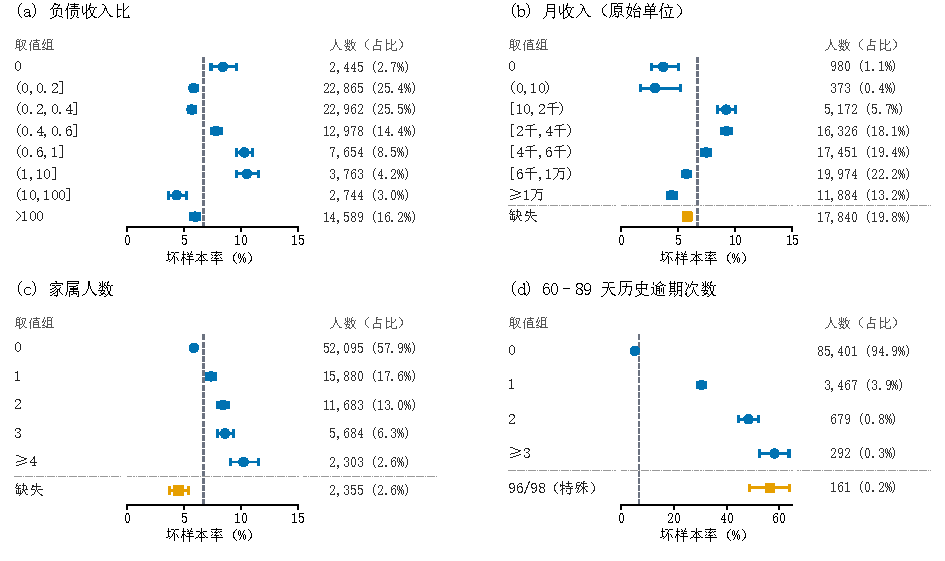
\includegraphics{figures/feature_risk.pdf}
  \small
  \caption{四变量的训练集分布与边际风险}
  \label{fig:training-feature-risk}
  \begin{minipage}{\linewidth}
    \footnotesize
    注：点为坏样本率，横线为记录层面的 Wilson 95\% 二项比例区间，
    右列为人数及占全部训练样本的比例。虚线为训练集总体坏样本率，
    方块标记缺失或 96/98 特殊组；各面板横轴范围不同。
  \end{minipage}
\end{figure}
